%======================================================================
\NEWSEC
%======================================================================

\subsection{\ssFields}

\begin{frame}[fragile,label=ss-fields] 
\secframetitle{\ssFields}
\greenbf{Field classes represent field data on \code{Block}s}
\ \\
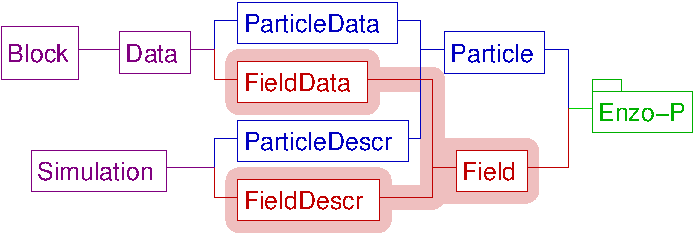
\includegraphics[width=2in]{data-classes-field.pdf}
\begin{itemize}
\item \greencode{FieldBlock}
\begin{itemize}
\item represents state-independent (intrinsic) data
\item associated with \greencode{Block}'s: one per mesh node
\end{itemize}
\item \greencode{FieldDescr}
\begin{itemize}
\item represents state-dependent (extrinsic) data
\item associated with \greencode{Simulation} object: one per process
\end{itemize}
\item Applications access field data via \greencode{Field} objects
\end{itemize}
\end{frame}

\begin{frame}[fragile] 
\secframetitle{\ssFields}
\greenbf{Field classes represent field data on \code{Block}s}
\ \\

\begin{itemize}
\item \greencode{FieldBlock}
\item precision, ghost depth, padding, alignment, centering
\end{itemize}
\end{frame}

%----------------------------------------------------------------------

\begin{frame}[fragile] 
\secframetitle{\ssFields}
\greenbf{Field class API: basic functions}
\footnotesize
\begin{semiverbatim}

   \comment{\# Return the number of fields}
   \type{int} \function{field_count} ();

   \comment{\# Return the integer handle for the named field.}
   \type{int} \function{field_id} (\variable{name});

   \comment{\# Return name of the ith field.}  
   \type{string} \function{field_name} (\variable{id});
 
\end{semiverbatim}
\end{frame}

%----------------------------------------------------------------------

\begin{frame}[fragile]
\secframetitle{\ssFields}
\greenbf{Field class API: accessing field data}
\footnotesize
\begin{semiverbatim}

   \comment{\# Return the array associated with the specified field}
   \type{char} * \function{values} (\variable{id});
   \type{char} * \function{values} (\variable{name});

   \comment{Return dimensions of fields on the data, assuming centered.}
   \keyword{void}  \function{dimensions} (\variable{id}, *\variable{mx}, *\variable{my}=\valuetext{0}, *\variable{mz}=\valuetext{0})

   \comment{\# Return size of fields on the data, assuming centered.}
   \keyword{void} \function{size} (*\variable{nx}, *\variable{ny}=\valuetext{0}, *\variable{nz}=\valuetext{0})

\end{semiverbatim}
\link{field-access}{Accessing field data is relatively easy}

\end{frame}

%----------------------------------------------------------------------

\begin{frame}[fragile]
\secframetitle{\ssFields}
\greenbf{Field class API: field characteristics}
\footnotesize
\begin{semiverbatim}

   \comment{\# Ghost depth of each field}
   \keyword{void} \function{set_ghost_depth} (\variable{id},  \variable{gx},  \variable{gy}=\valuetext{0},  \variable{gz}=\valuetext{0});
   \keyword{void} \function{ghost_depth}     (\variable{id}, *\variable{gx}, *\variable{gy}=\valuetext{0}, *\variable{gz}=\valuetext{0});

   \comment{\# Precision of each field: single, double, long double}
   \keyword{void} \function{set_precision} (\variable{id}, \variable{precision});
    \type{int} \function{precision}     (\variable{id});

   \comment{\# Cell centering of each field: -1, 0, or 1}
   \keyword{void} \function{set_centering} (\variable{id},  \variable{cx},  \variable{cy}=\valuetext{0},  \variable{cz}=\valuetext{0});
   \keyword{void} \function{centering}     (\variable{id}, *\variable{cx}, *\variable{cy}=\valuetext{0}, *\variable{cz}=\valuetext{0});

\end{semiverbatim}
\end{frame}

%----------------------------------------------------------------------

\begin{frame}[fragile]
\secframetitle{\ssFields}
\greenbf{Field class API: performance}
\footnotesize
\begin{semiverbatim}

   \comment{\# Byte alignment of field arrays in memory}
   \keyword{void} \function{set_alignment} (\variable{alignment});
    \type{int} \function{alignment} ();

   \comment{\# Byte padding between field arrays in memory}
   \keyword{void} \function{set_padding} (\variable{padding});
    \type{int} \function{padding} ();

\end{semiverbatim}
\end{frame}

%----------------------------------------------------------------------

\begin{frame}[fragile]
\secframetitle{\ssFields}
\greenbf{Field class API: fields can be associated with groups}
\footnotesize
\begin{semiverbatim}

   \comment{\# Return the Grouping object for the Fields}
   \type{Grouping} * \type{Field}::\function{groups} ();

   \comment{\# Add an item to a group. (Cello)}
   \keyword{void} \type{Grouping}::\function{add} (\variable{item}, \variable{group});
   
   \comment{\# Return whether the item is in the given Grouping.}
   \type{bool} \type{Grouping}::\function{is_in} (item, group)

   \comment{\# Return the number of items in the Grouping.}
   \type{int} \type{Grouping}::\function{size} (\variable{item})
   
   \comment{\# Return the ith Field in the Grouping.} 
   \type{string} \type{Grouping}::\function{item} (\variable{group}, \variable{i});

\end{semiverbatim}
\end{frame}

%   std::string field\_name(size\_t id) const throw(std::out\_of\_range)
% 
%   bool is\_field(const std::string \& name) const throw()
%   int field\_id(const std::string \& name) const throw()
%   Grouping * groups () 
%   void centering(int id, int * cx, int * cy = 0, int * cz = 0) const 
%   void ghosts(int id, int * gx, int * gy = 0, int * gz = 0) const 
%     throw(std::out\_of\_range)
%   int precision(int id) const throw(std::out\_of\_range)
%   int bytes\_per\_element(int id) const throw()
%   void size(int * nx, int * ny = 0, int * nz = 0) const throw()
%   void dimensions(int id\_field,int * mx, int * my = 0, int * mz = 0) const throw()
%   char * values (int id) throw (std::out\_of\_range)
%   char * unknowns ( int id) throw (std::out\_of\_range)
%   void cell\_width(double xm,   double xp,   double * hx,
% 		  double ym=0, double yp=0, double * hy=0,
% 		  double zm=0, double zp=0, double * hz=0) const throw ()
%   void clear ( float value = 0.0, 
% 	       int id\_first = -1, 
% 	       int id\_last  = -1) throw()
%   bool ghosts\_allocated() const throw ()
%   int field\_size (int id, int *nx=0, int *ny=0, int *nz=0) const throw()

%\end{frame}

